\documentclass{article}
\usepackage{graphicx}
\usepackage{amsmath}

\begin{document}

\title{Solutions to hw2 homework on Convex Optimization %https://web.stanford.edu/class/ee364a/homework.html}
\author{Andrei Keino}
\maketitle
% 3.2, 3.22, 3.28, 3.39, A2.23, A2.42, A2.46
\section*{3.1}
Suppose $f: R \rightarrow R$ is convex and $a, b \in \boldsymbol{dom} f$ with $a < b$. \\

(a) Show what \\
$f(x) \leq \frac{b - x}{b - a}f(a) + \frac{x - a}{b - a}f(b)$
for all $x \in [a, b]$\\

Definition of function convexity: \\

A function $f: R^n \rightarrow R$ is convex if $\boldsymbol{dom} f$ is a convex set \\ and for all $x, y \in \boldsymbol{dom} f$ and $0 \leq \theta \leq 1$ we have \\
$f(\theta x + (1 - \theta)y) \leq \theta f(x) + (1 - \theta) f(y)$ \\

Solution:\\

Let $z = \theta x + (1- \theta)y, \, $ let 
$z, x, y\in [a, b]$, \\
let $\theta = \frac{b - z}{b - a}$, 
then $1 - \theta = \frac{z - a}{b - a}$, \\therefore $\theta \in [0, 1]$. \\
Then by definition of convexity of $f$:\\
$$\boldsymbol{f(z)} = f(\theta x + (1- \theta)y) \leq 
\theta f(x) + (1 - \theta) f(y)  = 
\boldsymbol{\frac{b - z}{b - a} f(x) + \frac{z - a}{b - a} f(y)}$$
\\ and then for $x = a$, $y = b$ we have: \\
$$f(z) \leq \frac{b - z}{b - a} f(a) + \frac{z - a}{b - a} f(b)$$ (1)
\\ Proved. \\

(b) Show what \\
$$ \frac{f(x) - f(a)}{x - a} \leq \frac{f(b) - f(a)}{b - a} \leq \frac{f(b) - f(x)}{b - x}$$ \\

Solution: \\

First we show what $$ \frac{f(x) - f(a)}{x - a} \leq \frac{f(b) - f(a)}{b - a}$$ \\

Using the result from  the inequality proved in (a), dividing the right and left parts of the inequality  on $(x - a)$ and subtracting from the left and right parts of the inequality $\frac{f(a)}{x - a}$ we get $$ \frac{f(x) - f(a)}{x - a} \leq \frac{f(b) - f(a)}{b - a}$$\\

Now second part: Using the result from  the inequality proved in (a), dividing the right and left parts of the inequality  on $(b - x)$ and subtracting from the left and right parts of the inequality $\frac{f(b)}{b - x}$ we get $$ \frac{f(b) - f(a)}{b - a} \leq \frac{f(b) - f(x)}{b - x}$$\\
Proved.

\begin{figure}
	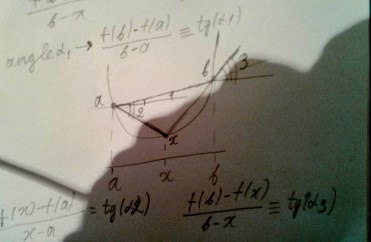
\includegraphics[width=\linewidth]
	{20200530_123213.jpg}
	\caption{A sketch.}
	\label{fig:picture}
\end{figure}

\end{document}

